% Midsem presentation, alpha-chess-rl (Monsoon 2026).
% Build:  cd reports/midsem/slides && latexmk -pdf midsem.tex
% Figures come from ../figures/ (team results) and diagrams/ (TikZ, shared with the docs).
\documentclass[aspectratio=169, 10pt]{beamer}
\usetheme[progressbar=frametitle, numbering=fraction, block=fill]{metropolis}
\usepackage{amsmath, amssymb}
\usepackage{booktabs}
\usepackage{graphicx}
\usepackage{tikz}
% Shared TikZ styles for the midsem diagrams (used by the slides and the standalone figures).
\usetikzlibrary{arrows.meta, positioning, fit, backgrounds, calc, shapes.geometric}

\definecolor{acNet}{HTML}{3A52C4}      % network / training (Samyak)
\definecolor{acSearch}{HTML}{C98410}   % search / evaluation (Agriya)
\definecolor{acDP}{HTML}{1F7A4B}       % exact endgames (Vatsl)
\definecolor{acData}{HTML}{6B4FA0}     % data
\definecolor{acInk}{HTML}{1B2330}
\definecolor{acMuted}{HTML}{5B6676}

\tikzset{
  box/.style={draw=#1, line width=0.9pt, rounded corners=3pt, fill=#1!8,
              align=center, inner sep=4pt, font=\footnotesize, text=acInk},
  box/.default=acInk,
  arr/.style={-{Stealth[length=2.4mm]}, line width=0.9pt, draw=acInk!80},
  lbl/.style={font=\scriptsize, text=acMuted, align=center},
  stage/.style={draw=acMuted!60, dashed, rounded corners=6pt, inner sep=7pt},
  stagetitle/.style={font=\scriptsize\bfseries, text=acMuted},
}

\graphicspath{{../figures/}{diagrams/}}

\setbeamercolor{progress bar}{fg=acNet}
\setbeamercolor{frametitle}{bg=acInk}
\setbeamercolor{alerted text}{fg=acSearch}

\newcommand{\track}[2]{{\color{#1}\textbf{#2}}}
\newcommand{\who}[2]{\hfill{\scriptsize\color{#1}#2}}
\newcommand{\figbox}[2]{% placeholder when a figure is not generated yet
  \begin{tikzpicture}\node[draw=acMuted, dashed, rounded corners, minimum width=#1,
    minimum height=0.6*#1, align=center, text=acMuted, font=\small]{#2};\end{tikzpicture}}

\title{AlphaChess-RL: a small AlphaZero-style chess engine}
\subtitle{Midsem progress: exact endgames, search, and the supervised start}
\author{Vatsl Goswami \and Agriya Yadav \and Samyak Baid}
\institute{Reinforcement Learning course project · Ashoka University · Monsoon 2026}
\date{14 October 2026}

\begin{document}

\maketitle

% ============================================================================================
\begin{frame}{The question}
  \small
  \begin{columns}[T]
    \begin{column}{0.56\textwidth}
      \textbf{Goal.} Build a chess agent the AlphaZero way, at student scale:
      \begin{enumerate}
        \item a \alert{policy--value network} learns from human games;
        \item \alert{MCTS self-play} improves it by reinforcement learning;
        \item we \alert{measure how much Elo the RL adds} on top of the supervised start.
      \end{enumerate}
      \medskip
      \textbf{Scope decisions} (to fit our compute):
      \begin{itemize}
        \item self-play only from \textbf{French Defense} openings;
        \item games stop at \textbf{$\le$ 5 pieces} and take the exact tablebase result;
        \item the supervised stage still covers all of chess.
      \end{itemize}
    \end{column}
    \begin{column}{0.4\textwidth}
      \begin{block}{Three tracks}
        \track{acDP}{Vatsl}: exact endgame DP, tablebases, Lichess data\\[3pt]
        \track{acSearch}{Agriya}: MCTS and the evaluation harness\\[3pt]
        \track{acNet}{Samyak}: encoding, network, training
      \end{block}
      \medskip
      {\small Weakness in non-French openings and in endgames the network never trains on is
      \emph{expected}, not a bug.}
    \end{column}
  \end{columns}
\end{frame}

% ============================================================================================
\begin{frame}{Chess as an MDP}
  \small
  \begin{columns}[T]
    \begin{column}{0.52\textwidth}
      \begin{itemize}
        \item \textbf{State} $s$: the position plus whose turn it is.
        \item \textbf{Action} $a$: a legal move. \textbf{Transition}: deterministic.
        \item \textbf{Reward}: only at the end: $+1$ win, $0$ draw, $-1$ loss.
        \item Two players, zero-sum, so we store every value \alert{from the side to move's
          point of view}.
      \end{itemize}
      \medskip
      One rule covers both players (\textbf{negamax Bellman}):
      \[
        V(s) \;=\; \max_{a \in A(s)} \; -\,\gamma\, V\big(f(s,a)\big)
      \]
      The minus sign means ``switch seats'': good for my opponent is bad for me.
    \end{column}
    \begin{column}{0.44\textwidth}
      \begin{block}{One convention, everywhere}
        \small
        Endgame tables, MCTS backups, the network's value head and the training targets all
        use \emph{side-to-move} values in $[-1,1]$.\\[4pt]
        The board encoding flips the board when Black moves, so the network always sees
        ``my pieces moving up''.
      \end{block}
      \medskip
      {\small With $\gamma = 0.9$: mate in $d$ plies is worth $\pm\gamma^{d}$, so the winner
      prefers faster mates and the loser longer resistance.}
    \end{column}
  \end{columns}
\end{frame}

% ============================================================================================
\begin{frame}{The whole pipeline}
  \centering
  \resizebox{\textwidth}{!}{% The full training pipeline: supervised start (stage 1), then the self-play RL loop (stage 2)
% with the tablebase cut-off at 5 or fewer pieces. Colours: blue = network/training (Samyak),
% orange = search/evaluation (Agriya), green = exact endgames (Vatsl), purple = data.
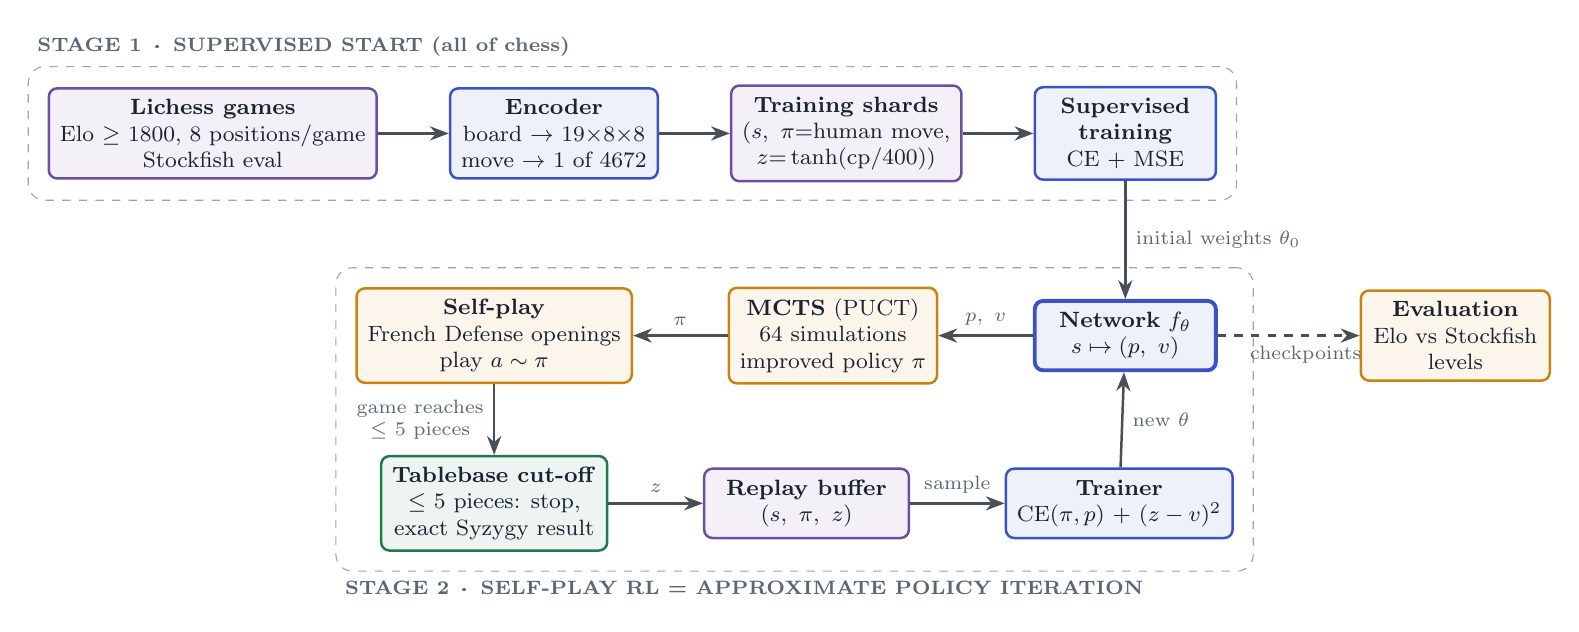
\begin{tikzpicture}[node distance=6mm and 9mm]
  % ---------------- Stage 1: supervised start ----------------
  \node[box=acData, minimum width=2.6cm] (lichess)
    {\textbf{Lichess games}\\Elo $\ge$ 1800, 8 positions/game\\Stockfish eval};
  \node[box=acNet, right=of lichess, minimum width=2.4cm] (enc)
    {\textbf{Encoder}\\board $\to$ 19$\times$8$\times$8\\move $\to$ 1 of 4672};
  \node[box=acData, right=of enc, minimum width=2.6cm] (shards)
    {\textbf{Training shards}\\$(s,\ \pi{=}\text{human move},$\\$z{=}\tanh(\text{cp}/400))$};
  \node[box=acNet, right=of shards, minimum width=2.3cm] (sltrain)
    {\textbf{Supervised}\\\textbf{training}\\CE $+$ MSE};
  \draw[arr] (lichess) -- (enc);
  \draw[arr] (enc) -- (shards);
  \draw[arr] (shards) -- (sltrain);

  % ---------------- Stage 2: self-play RL loop ----------------
  \node[box=acNet, below=15mm of sltrain, minimum width=2.3cm, line width=1.4pt] (net)
    {\textbf{Network} $f_\theta$\\$s \mapsto (p,\ v)$};
  \node[box=acSearch, left=12mm of net, minimum width=2.6cm] (mcts)
    {\textbf{MCTS} (PUCT)\\64 simulations\\improved policy $\pi$};
  \node[box=acSearch, left=12mm of mcts, minimum width=2.7cm] (selfplay)
    {\textbf{Self-play}\\French Defense openings\\play $a \sim \pi$};
  \node[box=acDP, below=9mm of selfplay, minimum width=2.7cm] (tb)
    {\textbf{Tablebase cut-off}\\$\le$ 5 pieces: stop,\\exact Syzygy result};
  \node[box=acData, right=12mm of tb, minimum width=2.6cm] (replay)
    {\textbf{Replay buffer}\\$(s,\ \pi,\ z)$};
  \node[box=acNet, right=12mm of replay, minimum width=2.3cm] (rltrain)
    {\textbf{Trainer}\\CE$(\pi, p)$ $+$ $(z-v)^2$};

  \draw[arr] (sltrain) -- node[lbl, right] {initial weights $\theta_0$} (net);
  \draw[arr] (net) -- node[lbl, above] {$p,\ v$} (mcts);
  \draw[arr] (mcts) -- node[lbl, above] {$\pi$} (selfplay);
  \draw[arr] (selfplay) -- node[lbl, left] {game reaches\\$\le$ 5 pieces} (tb);
  \draw[arr] (tb) -- node[lbl, above] {$z$} (replay);
  \draw[arr] (replay) -- node[lbl, above] {sample} (rltrain);
  \draw[arr] (rltrain) -- node[lbl, right] {new $\theta$} (net);

  % ---------------- Evaluation ----------------
  \node[box=acSearch, right=18mm of net, minimum width=2.4cm] (eval)
    {\textbf{Evaluation}\\Elo vs Stockfish\\levels};
  \draw[arr, dashed] (net) -- node[lbl, below, pos=0.62] {checkpoints} (eval);

  % Stage frames
  \begin{scope}[on background layer]
    \node[stage, fit=(lichess)(sltrain)] (s1) {};
    \node[stage, fit=(selfplay)(tb)(rltrain)(net)] (s2) {};
  \end{scope}
  \node[stagetitle, anchor=south west] at (s1.north west) {STAGE 1 \,·\, SUPERVISED START (all of chess)};
  \node[stagetitle, anchor=north west] at (s2.south west) {STAGE 2 \,·\, SELF-PLAY RL = APPROXIMATE POLICY ITERATION};
\end{tikzpicture}
}\\[2pt]
  {\scriptsize Colours: \track{acNet}{network / training} · \track{acSearch}{search /
  evaluation} · \track{acDP}{exact endgames} · \track{acData}{data}}
\end{frame}

% ============================================================================================
\begin{frame}{Where we are (Phase 1)}
  \centering
  \small
  \begin{tabular}{@{}lll@{}}
    \toprule
    Track & Done & Next \\
    \midrule
    \track{acDP}{Exact endgame DP} & KQK, KRK, KPK solved and verified 100\% vs Syzygy; & full 2M-position \\
     & VI vs retrograde vs RTDP; approximation study & Lichess run \\
    \track{acDP}{Lichess data} & streaming, filtering, sampling, Parquet shards & \\
    \midrule
    \track{acSearch}{MCTS} & batched PUCT, Gumbel root variant, UCI engine & Elo vs simulations \\
    \track{acSearch}{Evaluation} & paired matches, Stockfish, Elo with bootstrap CIs, & with the real \\
     & puzzle and centipawn-loss metrics & network \\
    \midrule
    \track{acNet}{Encoding} & 19 board planes, 4672-move index, legal mask & \\
    \track{acNet}{Network} & 6-block ResNet, policy + value heads (505k params) & train on 2M \\
    \track{acNet}{Training} & supervised trainer; trial run on 5k positions works & positions \\
    \bottomrule
  \end{tabular}
  \medskip

  All parts meet at the shared interfaces (\texttt{docs/INTERFACES.md}): \textbf{402 tests pass}.
\end{frame}

% ============================================================================================
\section{Exact endgames by dynamic programming · Vatsl}

\begin{frame}{Endgames as a shortest-path problem}
  \begin{columns}[T]
    \begin{column}{0.55\textwidth}
      KQK, KRK, KPK: every position, both sides to move.
      \begin{itemize}
        \item \textbf{Value iteration}: back up every position every sweep until nothing
          changes. KRK: 33 sweeps, \textbf{1.65M} backups.
        \item \textbf{Retrograde analysis}: walk backwards from the mates, one DTM level at a
          time; each move is walked once. KRK: \textbf{0.52M} steps.
        \item \textbf{Symmetry}: 8 board symmetries (pawnless) shrink KQK/KRK to 81,920
          slots instead of 524,288.
      \end{itemize}
      \medskip
      Tables store win/draw/loss + plies to mate (DTM) + the best move.
    \end{column}
    \begin{column}{0.42\textwidth}
      \small
      \begin{tabular}{@{}lrr@{}}
        \toprule
        Table & Positions & Longest mate \\
        \midrule
        KQK & 46,137 & mate in 10 \\
        KRK & 50,015 & mate in 16 \\
        KPK & 165,676 & mate in 28 \\
        \bottomrule
      \end{tabular}\\[6pt]
      {\scriptsize Solve time: KQK 3.0 s, KRK 2.8 s, KPK 11.1 s on one CPU core. All three
      longest mates match the known values.}
    \end{column}
  \end{columns}
\end{frame}

\begin{frame}{Exact tables, fully verified}
  \begin{columns}[c]
    \begin{column}{0.55\textwidth}
      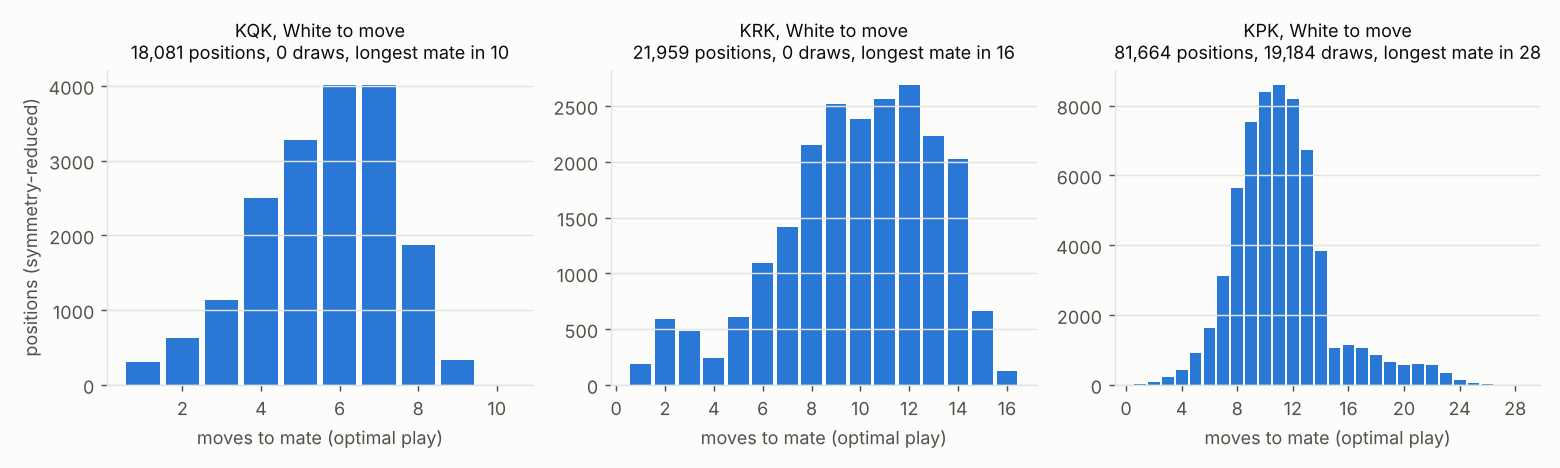
\includegraphics[width=\textwidth]{dtm_histograms.png}
    \end{column}
    \begin{column}{0.42\textwidth}
      \small
      \textbf{Verification, every legal position:}
      \begin{itemize}
        \item win/draw/loss agrees with \textbf{Syzygy 100\%} on all three tables;
        \item every value satisfies the negamax Bellman equation;
        \item an independent value iteration reproduces WDL and DTM exactly;
        \item Stockfish (1,000 positions per table) never found a shorter mate.
      \end{itemize}
    \end{column}
  \end{columns}
\end{frame}

\begin{frame}{KPK: the textbook results fall out of the DP}
  \begin{columns}[c]
    \begin{column}{0.55\textwidth}
      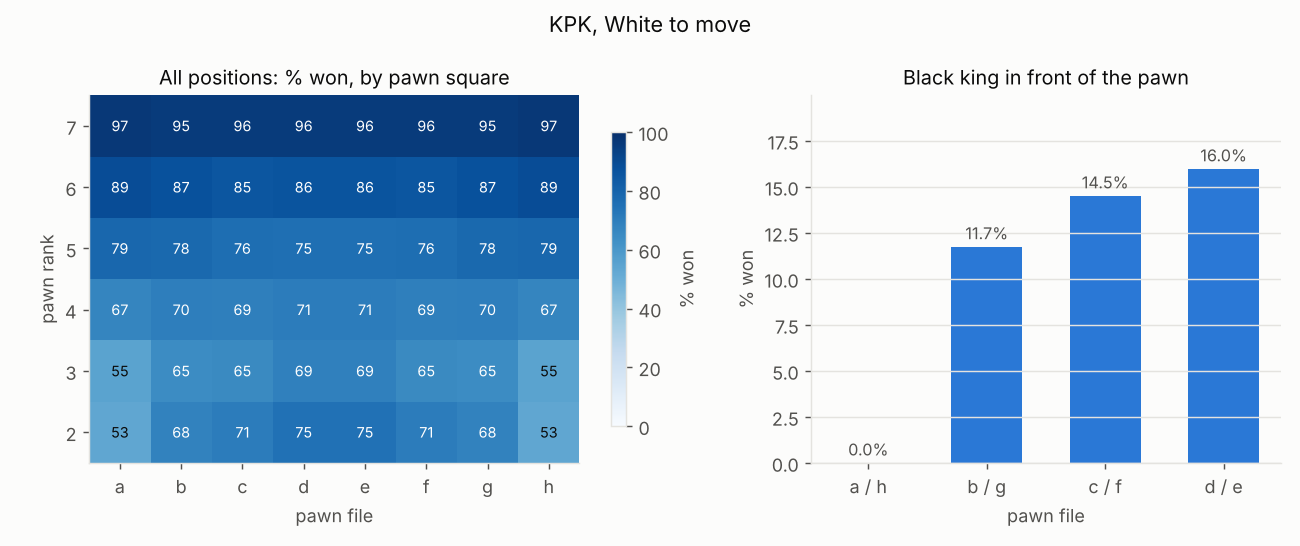
\includegraphics[width=\textwidth]{kpk_win_by_pawn_square.png}
    \end{column}
    \begin{column}{0.42\textwidth}
      \small
      \begin{itemize}
        \item White to move wins \textbf{76.5\%} of KPK positions.
        \item The pawn's rank matters most: 53--75\% won on rank 2, 96--97\% on rank 7.
        \item \textbf{Rook pawn, defender in front: 0\% won}, against 12--16\% for b-, c-,
          d-pawns. Exactly the textbook rule.
      \end{itemize}
    \end{column}
  \end{columns}
\end{frame}

\begin{frame}{RTDP: only back up what play actually reaches}
  \begin{columns}[c]
    \begin{column}{0.52\textwidth}
      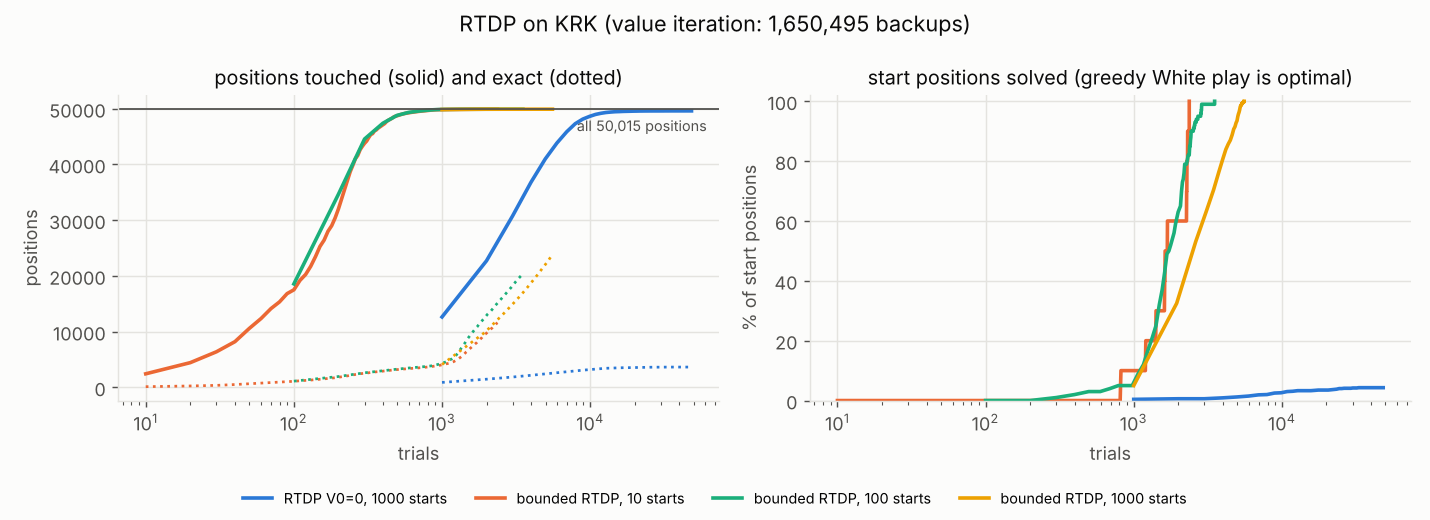
\includegraphics[width=\textwidth]{rtdp_touched_vs_trials.png}
    \end{column}
    \begin{column}{0.45\textwidth}
      \small
      \begin{itemize}
        \item \textbf{Finding}: plain RTDP with $V_0 = 0$ \alert{does not converge} on KRK.
          0 is pessimistic for White (every position is won), so White stops exploring.
        \item \textbf{Fix}: keep an upper and a lower bound per position, so both sides stay
          optimistic. Converges with 37--41\% of value iteration's backups.
        \item On a graph this small RTDP still touches almost every position. Its savings
          need a bigger space or narrow starts: exactly our French-only self-play setting.
      \end{itemize}
    \end{column}
  \end{columns}
\end{frame}

\begin{frame}{How well can a network learn an exact value? (KRK)}
  \begin{columns}[c]
    \begin{column}{0.5\textwidth}
      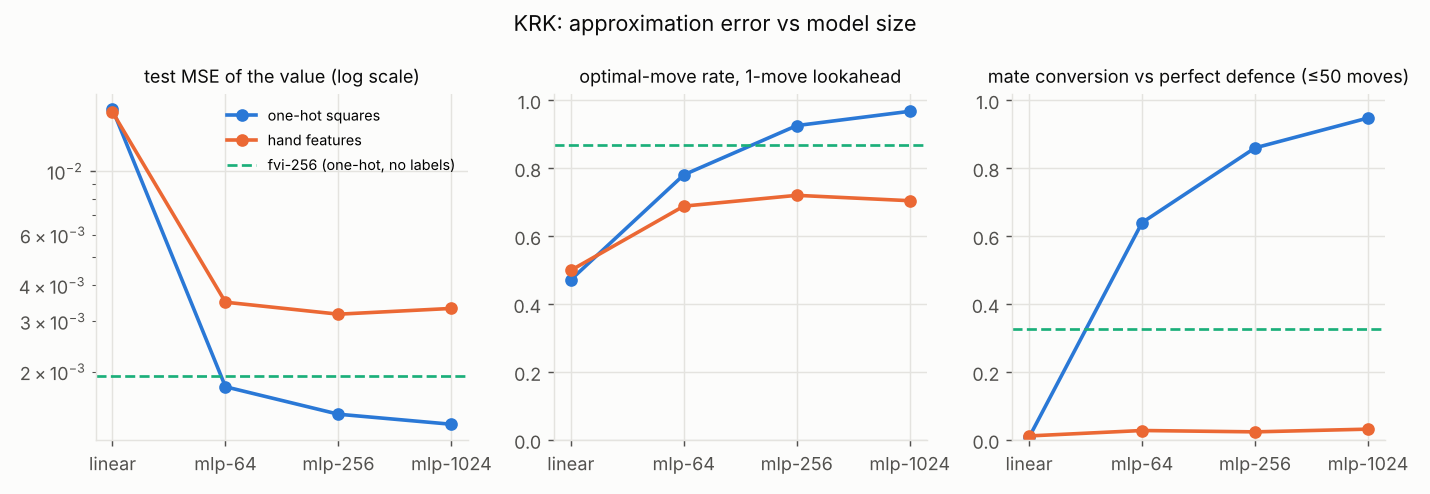
\includegraphics[width=\textwidth]{approx_error_vs_size.png}
    \end{column}
    \begin{column}{0.47\textwidth}
      \scriptsize
      \resizebox{\linewidth}{!}{%
      \begin{tabular}{@{}llrr@{}}
        \toprule
        Model & Inputs & Optimal move & Mate conv. \\
        \midrule
        MLP-64 & one-hot & 78.1\% & 64.0\% \\
        MLP-1024 & one-hot & 96.8\% & \textbf{94.8\%} \\
        MLP-1024 & hand features & 70.5\% & 3.2\% \\
        FVI-256 (no labels) & one-hot & 86.9\% & 32.8\% \\
        \bottomrule
      \end{tabular}}\\[6pt]
      \small
      \begin{itemize}
        \item \textbf{Raw inputs + capacity beat hand features}: features know \emph{who}
          wins, not \emph{how}. This is the bet behind our big network.
        \item Bootstrapping without labels (fitted VI) drifts far from the mates.
        \item Errors compound over long mates: one wrong move in 16 loses the win.
      \end{itemize}
    \end{column}
  \end{columns}
\end{frame}

% ============================================================================================
\section{Search and evaluation · Agriya}

\begin{frame}{MCTS with PUCT}
  \begin{columns}[T]
    \begin{column}{0.55\textwidth}
      Each simulation:
      \begin{enumerate}
        \item \textbf{Select} down the tree by
          \[
            Q(a) + c_{\text{puct}}\, P(a)\, \frac{\sqrt{N_{\text{parent}}+1}}{1 + N(a)}
          \]
        \item \textbf{Expand} a new position: the network gives priors $P$ and value $v$.
        \item \textbf{Evaluate}: rules for mate/stalemate, else $v$.
        \item \textbf{Back up} to the root, \alert{negating at every move}.
      \end{enumerate}
      The root's visit counts $\pi(a) \propto N(a)$ are the \textbf{improved policy}.
    \end{column}
    \begin{column}{0.41\textwidth}
      \begin{block}{Engineering}
        \small
        \begin{itemize}
          \item batched leaf evaluation (GPU-friendly)
          \item legal priors only; malformed priors fall back to uniform
          \item visit counts sum exactly to the budget
          \item root Dirichlet noise for self-play; Gumbel root variant for low budgets
          \item tested: mate-in-one, backup signs, batching, terminal handling
        \end{itemize}
      \end{block}
    \end{column}
  \end{columns}
\end{frame}

\begin{frame}{Search turns an approximate value into a better policy}
  \begin{columns}[c]
    \begin{column}{0.52\textwidth}
      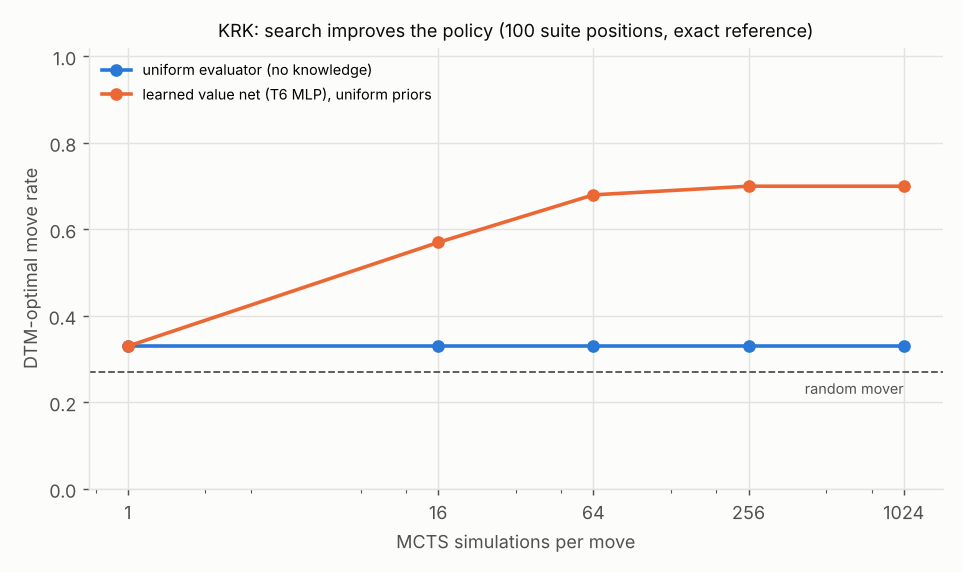
\includegraphics[width=\textwidth]{mcts_vs_sims_krk.png}
    \end{column}
    \begin{column}{0.45\textwidth}
      \small
      100 KRK positions, scored against the \textbf{exact} tables (DTM-optimal move rate):
      \medskip

      \begin{tabular}{@{}lrrr@{}}
        \toprule
        Simulations & 1 & 64 & 1024 \\
        \midrule
        Uniform evaluator & 33\% & 33\% & 33\% \\
        Learned value (MLP-64) & 33\% & 68\% & 70\% \\
        \bottomrule
      \end{tabular}\\[6pt]
      \begin{itemize}
        \item With no knowledge, search can't see 10--32-ply mates: it stays flat.
        \item With an imperfect learned value, search \alert{doubles} the optimal-move rate.
        \item This is AlphaZero's \textbf{policy-improvement step}, checked against ground
          truth.
      \end{itemize}
    \end{column}
  \end{columns}
\end{frame}

\begin{frame}{Evaluation harness: measuring Elo honestly}
  \begin{columns}[T]
    \begin{column}{0.5\textwidth}
      \begin{itemize}
        \item \textbf{UCI engine}: our agent speaks the standard chess-engine protocol.
        \item \textbf{Paired matches}: every opening played twice, colours swapped.
        \item \textbf{Stockfish} at fixed Elo levels (1350, 1500, 1700, 1900).
        \item \textbf{Elo} $= 400 \log_{10}\frac{\text{score}}{1-\text{score}}$ with 95\%
          bootstrap intervals over \emph{opening pairs}.
        \item Extra diagnostics: top-move agreement, centipawn loss, Lichess puzzles.
      \end{itemize}
    \end{column}
    \begin{column}{0.46\textwidth}
      \centering
      \IfFileExists{../figures/elo_vs_simulations.png}{%
        \includegraphics[width=\textwidth]{elo_vs_simulations.png}%
      }{%
        \figbox{6cm}{Elo vs simulations (0, 1, 16, 64, 256)\\[2pt]
        same checkpoint, openings, seeds\\[2pt]\textbf{runs with the first trained network}}%
      }
    \end{column}
  \end{columns}
\end{frame}

% ============================================================================================
\section{Encoding, network and training · Samyak}

\begin{frame}{Board encoding: what the network sees}
  \begin{columns}[T]
    \begin{column}{0.5\textwidth}
      A position becomes a stack of \textbf{19 planes of 8$\times$8}:
      \medskip

      \small
      \begin{tabular}{@{}rl@{}}
        \toprule
        Planes & Meaning \\
        \midrule
        0--5 & my P, N, B, R, Q, K \\
        6--11 & opponent's P, N, B, R, Q, K \\
        12 & repetition (seen before?) \\
        13--16 & castling rights, mine and theirs \\
        17 & colour to move \\
        18 & fifty-move counter / 100 \\
        \bottomrule
      \end{tabular}
    \end{column}
    \begin{column}{0.46\textwidth}
      \begin{block}{Always the side to move's view}
        \small
        If Black is to move, the board is \textbf{mirrored top-to-bottom} and colours swapped.
        So ``my pieces'' are always planes 0--5 and always move ``up''.\\[4pt]
        One network for both colours, and its value output is automatically from the mover's
        side, matching the negamax convention.
      \end{block}
      {\small Example: after 1.\,e4, Black's pawns appear on ``rank 2'' of planes 0, and
      White's e4-pawn appears on ``rank 5'' of plane 6.}
    \end{column}
  \end{columns}
\end{frame}

\begin{frame}{Move encoding: 4672 = 64 from-squares $\times$ 73 move types}
  \begin{columns}[T]
    \begin{column}{0.52\textwidth}
      \[
        \text{index} = \text{from\_square} \times 73 + \text{move\_type}
      \]
      \begin{itemize}
        \item \textbf{0--55}: queen-like, 8 directions $\times$ 7 distances (also king,
          pawn, castling, queen promotion)
        \item \textbf{56--63}: the 8 knight jumps
        \item \textbf{64--72}: underpromotions to N, B, R $\times$ 3 directions
      \end{itemize}
      Illegal entries are masked to $-\infty$ before the softmax.
    \end{column}
    \begin{column}{0.44\textwidth}
      \begin{block}{Worked examples (start position)}
        \small
        \textbf{e2e4}: from e2 = square 12, north (dir 0), distance 2 $\Rightarrow$ type 1\\
        index $= 12 \times 73 + 1 = \mathbf{877}$\\[4pt]
        \textbf{g1f3}: from g1 = square 6, knight jump $(-1,+2)$ = type 63\\
        index $= 6 \times 73 + 63 = \mathbf{501}$\\[4pt]
        \textbf{1\ldots e5} for Black is \emph{also} 877, because the board is flipped.
      \end{block}
      {\scriptsize Tested: every legal move in 308 positions maps to a unique index and back.}
    \end{column}
  \end{columns}
\end{frame}

\begin{frame}{The policy--value network}
  \centering
  \resizebox{\textwidth}{!}{% The policy-value ResNet (alphachess/model/net.py), default size 6 blocks x 64 channels.
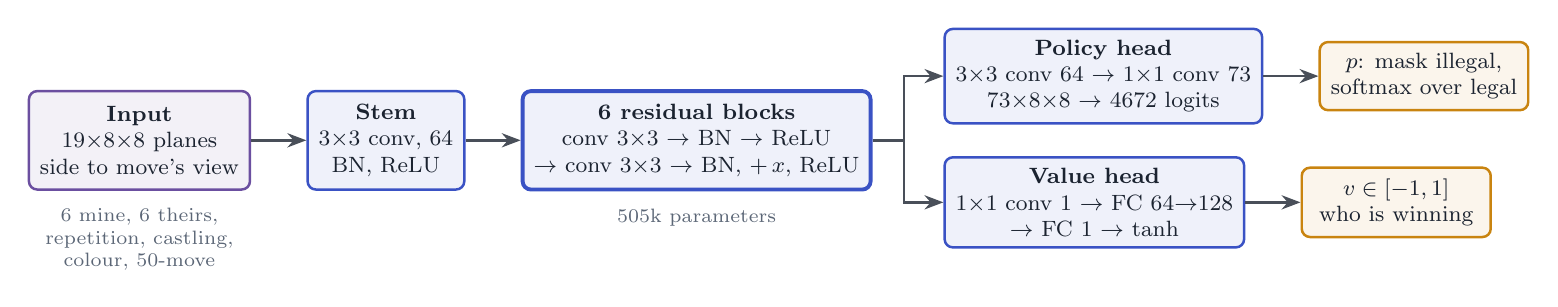
\begin{tikzpicture}[node distance=5mm and 7mm]
  \node[box=acData, minimum width=2.1cm, minimum height=1.25cm] (in)
    {\textbf{Input}\\19$\times$8$\times$8 planes\\side to move's view};
  \node[box=acNet, right=of in, minimum width=1.9cm, minimum height=1.25cm] (stem)
    {\textbf{Stem}\\3$\times$3 conv, 64\\BN, ReLU};
  \node[box=acNet, right=of stem, minimum width=2.9cm, minimum height=1.25cm,
        line width=1.4pt] (tower)
    {\textbf{6 residual blocks}\\conv 3$\times$3 $\to$ BN $\to$ ReLU\\$\to$ conv 3$\times$3 $\to$ BN, $+\,x$, ReLU};
  \node[box=acNet, above right=2mm and 9mm of tower.east, anchor=south west,
        minimum width=3.5cm] (phead)
    {\textbf{Policy head}\\3$\times$3 conv 64 $\to$ 1$\times$1 conv 73\\73$\times$8$\times$8 $\to$ 4672 logits};
  \node[box=acNet, below right=2mm and 9mm of tower.east, anchor=north west,
        minimum width=3.5cm] (vhead)
    {\textbf{Value head}\\1$\times$1 conv 1 $\to$ FC 64$\to$128\\$\to$ FC 1 $\to$ $\tanh$};
  \node[box=acSearch, right=of phead, minimum width=2.4cm] (pout)
    {$p$: mask illegal,\\softmax over legal};
  \node[box=acSearch, right=of vhead, minimum width=2.4cm] (vout)
    {$v \in [-1, 1]$\\who is winning};

  \draw[arr] (in) -- (stem);
  \draw[arr] (stem) -- (tower);
  \draw[arr] (tower.east) -- ++(4mm,0) |- (phead.west);
  \draw[arr] (tower.east) -- ++(4mm,0) |- (vhead.west);
  \draw[arr] (phead) -- (pout);
  \draw[arr] (vhead) -- (vout);

  \node[lbl, below=1mm of tower] {505k parameters};
  \node[lbl, below=1mm of in] {6 mine, 6 theirs,\\repetition, castling,\\colour, 50-move};
\end{tikzpicture}
}
  \bigskip

  \begin{columns}[T]
    \begin{column}{0.47\textwidth}
      \small
      \textbf{Policy head is convolutional}: plane $t$ at square $s$ is the logit of move type
      $t$ from $s$. Flattening gives index $s \cdot 73 + t$, exactly the move encoding.
    \end{column}
    \begin{column}{0.47\textwidth}
      \small
      \textbf{Value head} squashes to $[-1, 1]$ with $\tanh$: the expected result for the side
      to move. Plugs straight into Agriya's MCTS (tested).
    \end{column}
  \end{columns}
\end{frame}

\begin{frame}{Supervised training on Lichess}
  \begin{columns}[T]
    \begin{column}{0.52\textwidth}
      \textbf{Data} (Lichess, January 2024):
      \begin{itemize}
        \item rated games, both players $\ge$ 1800, no bullet, with Stockfish evals;
        \item 8 positions per game after move 4, split train/val/test by game;
        \item target move $\pi$ = the human's move (one-hot);
        \item target value $z = \tanh(\text{cp}/400)$, mate $\to \pm 1$, side to move's view.
      \end{itemize}
    \end{column}
    \begin{column}{0.44\textwidth}
      \textbf{Loss} (AlphaZero's, weight decay via AdamW):
      \[
        \mathcal{L} = \underbrace{-\textstyle\sum_a \pi(a)\log p_\theta(a\,|\,s)}_{\text{policy
        cross-entropy}} + \underbrace{(z - v_\theta(s))^2}_{\text{value MSE}}
      \]
      \small
      Shards stream one at a time, so memory stays flat as the dataset grows.
      Checkpoints, metrics and curves are written automatically.
    \end{column}
  \end{columns}
\end{frame}

\begin{frame}{Trial run: the training loop works end to end}
  \centering
  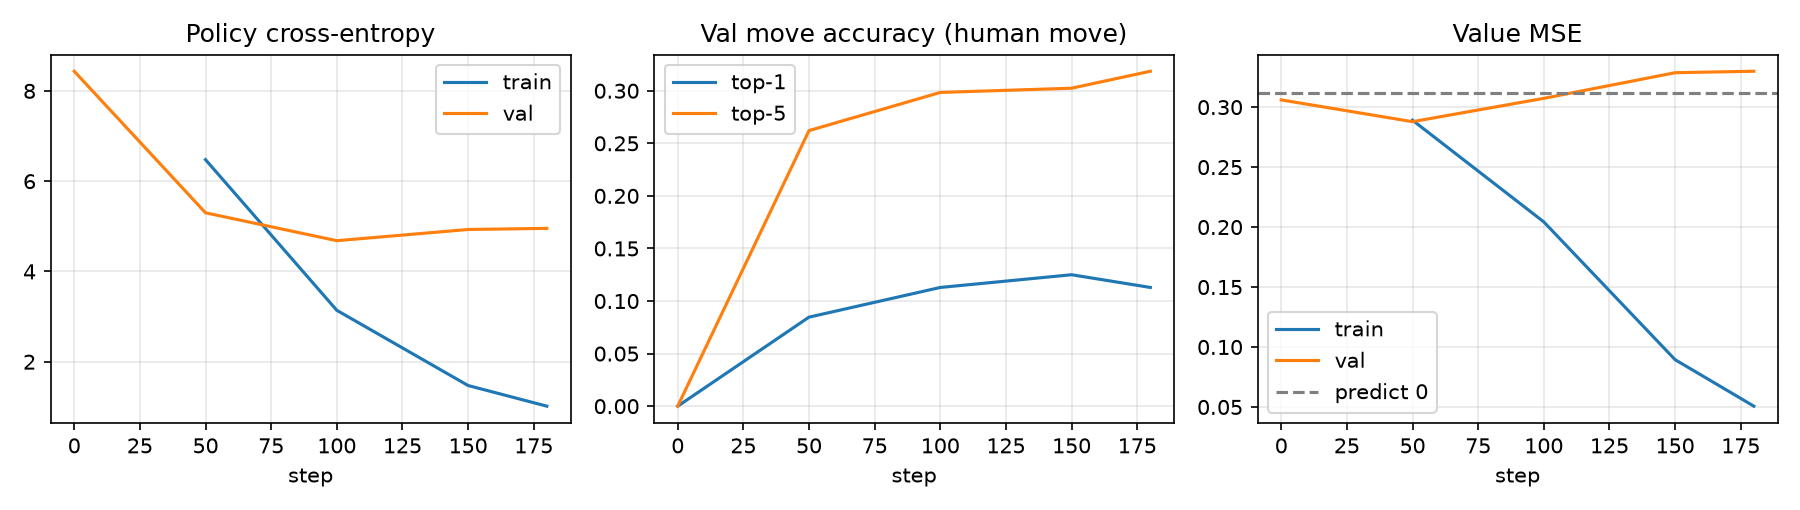
\includegraphics[width=0.95\textwidth]{sl_trial_5k_curves.png}\\[2pt]
  \begin{columns}[T]
    \begin{column}{0.48\textwidth}
      \small
      4,456 train / 248 val positions (625 games), 6$\times$64 ResNet, 10 epochs,
      \textbf{25 s on a MacBook Air GPU}.\\
      Val top-1 \textbf{0\% $\to$ 11\%}, top-5 \textbf{0\% $\to$ 32\%}
      (random legal move $\approx$ 3\%).
    \end{column}
    \begin{column}{0.48\textwidth}
      \small
      As expected at this size: the net \alert{memorises} (train CE 1.1 vs val 5.0) and the
      value head does not beat predicting 0 yet (0.33 vs 0.31). Judging who is winning needs
      far more data $\Rightarrow$ the 2M-position run.
    \end{column}
  \end{columns}
\end{frame}

% ============================================================================================
\section{Methodology going forward}

\begin{frame}{Step 1: supervised training at scale}
  \begin{itemize}
    \item \textbf{2M positions} from Lichess 2024-01 ($\approx$ 450$\times$ the trial run),
      encoded with the same pipeline.
    \item Train on the shared \textbf{2$\times$H100} workstation; same trainer, same
      checkpoints.
    \item Watch validation curves for overfitting; scale the network (e.g. 10 blocks
      $\times$ 128 channels) once the data supports it.
    \item \textbf{Deliverables}: val move accuracy, value error vs the predict-0 baseline, and
      the first \textbf{Elo vs simulations} plot with Agriya's harness.
  \end{itemize}
  \medskip
  \begin{block}{Why start supervised?}
    A random network makes MCTS no better than chance (the flat 33\% line). Human games give a
    sensible starting policy and value, so self-play starts from real chess.
  \end{block}
\end{frame}

\begin{frame}{Step 2: self-play RL as approximate policy iteration}
  \begin{columns}[T]
    \begin{column}{0.52\textwidth}
      Repeat:
      \begin{enumerate}
        \item \textbf{Policy improvement (search)}: MCTS from each position, guided by
          $(p_\theta, v_\theta)$, returns visit counts $\pi$, a \emph{better} policy than
          $p_\theta$.
        \item \textbf{Play}: self-play games from French Defense openings, moves sampled from
          $\pi$.
        \item \textbf{Policy evaluation (outcome)}: each game ends in a result $z$; games
          reaching $\le 5$ pieces take the \emph{exact} tablebase value.
        \item \textbf{Training stores the improvement}: fit $p_\theta \to \pi$ and
          $v_\theta \to z$ on the replay buffer.
      \end{enumerate}
    \end{column}
    \begin{column}{0.44\textwidth}
      \begin{block}{Policy iteration, with a network}
        \small
        Classic PI alternates evaluation and greedy improvement over a table.\\[3pt]
        Here the ``greedy step'' is search, and the network is a compressed, approximate
        table, so it is \textbf{approximate} PI (Bertsekas \& Tsitsiklis).\\[3pt]
        Vatsl's KRK result shows the improvement step working: 33\% $\to$ 70\%.
      \end{block}
      {\small The tablebase cut-off gives exact $z$ in endgames and shortens games.}
    \end{column}
  \end{columns}
\end{frame}

\begin{frame}{Evaluation plan}
  \begin{columns}[T]
    \begin{column}{0.5\textwidth}
      \textbf{Three curves}
      \begin{enumerate}
        \item \textbf{Elo vs Stockfish levels} 1350 / 1500 / 1700 / 1900 for the supervised
          and the RL network.
        \item \textbf{Elo vs MCTS simulations} 0, 1, 16, 64, 256 with a fixed checkpoint.
        \item \textbf{Elo vs training iterations} during self-play: does RL keep adding Elo?
      \end{enumerate}
    \end{column}
    \begin{column}{0.46\textwidth}
      \textbf{Protocol}
      \begin{itemize}
        \small
        \item frozen checkpoint, openings, seeds, Stockfish settings
        \item pilot 20--40 games, then 200 games per point
        \item colour-swapped pairs; 95\% bootstrap intervals
        \item no claims where intervals overlap
        \item supporting: puzzles, top-move agreement, centipawn loss
      \end{itemize}
    \end{column}
  \end{columns}
\end{frame}

\begin{frame}{Ablations}
  \small
  \begin{tabular}{@{}p{0.45\textwidth}p{0.5\textwidth}@{}}
    \toprule
    Ablation & What it tells us \\
    \midrule
    Supervised only vs supervised + RL & the headline: how much Elo self-play adds \\
    MCTS budget in self-play (16 / 64 / 256) & how much search quality drives the RL gain \\
    Tablebase cut-off on vs off & does exact endgame adjudication help learning? \\
    Value target: game result $z$ vs blended with search $Q$ & noise vs bias in value targets \\
    Network size (6$\times$64 vs 10$\times$128) & capacity vs data \\
    PUCT vs Gumbel root at low budgets & better policy improvement with few simulations? \\
    French-only vs held-out openings & how far the RL gains transfer \\
    \bottomrule
  \end{tabular}
\end{frame}

\begin{frame}{Next steps}
  \begin{columns}[T]
    \begin{column}{0.32\textwidth}
      \track{acDP}{Vatsl}
      \begin{itemize}
        \small
        \item full 2M-position Lichess run and encoding
        \item replay buffer, self-play workers, tablebase adjudication
      \end{itemize}
    \end{column}
    \begin{column}{0.32\textwidth}
      \track{acSearch}{Agriya}
      \begin{itemize}
        \small
        \item Elo vs simulations with the trained network
        \item rate every RL checkpoint in the same harness
      \end{itemize}
    \end{column}
    \begin{column}{0.32\textwidth}
      \track{acNet}{Samyak}
      \begin{itemize}
        \small
        \item long supervised run on the H100s
        \item RL trainer: $(s, \pi, z)$ from the replay buffer
        \item checkpoint schedule for self-play
      \end{itemize}
    \end{column}
  \end{columns}
  \bigskip
  \begin{block}{Summary}
    The three pieces are built and connected: exact endgames (verified 100\%), batched MCTS
    with an honest Elo harness, and an encoder + network + trainer that learns on real data.
    Next: train at scale, then let search teach the network.
  \end{block}
\end{frame}

\begin{frame}[standout]
  Questions?
\end{frame}

\end{document}
